% SPI modultest

\subsection{API}

APIen testes med en Logic-Analyzer koblet på \verb+MOSI+, \verb+CLK+ og \verb+ENABLE+ benene på Devkit8000. Der køres derefter et testprogram, hvor hver enkelt metode testes.


% Aktiver
\subsubsection*{Aktiver}

Aktiver testes med et testobjekt

\begin{lstlisting}[language=C]
int main(void){
	SPI_api test;
	test.activate(1); // 1 er et dummy enhedsnummer
}
\end{lstlisting}

\begin{figure}[H]
\centering
{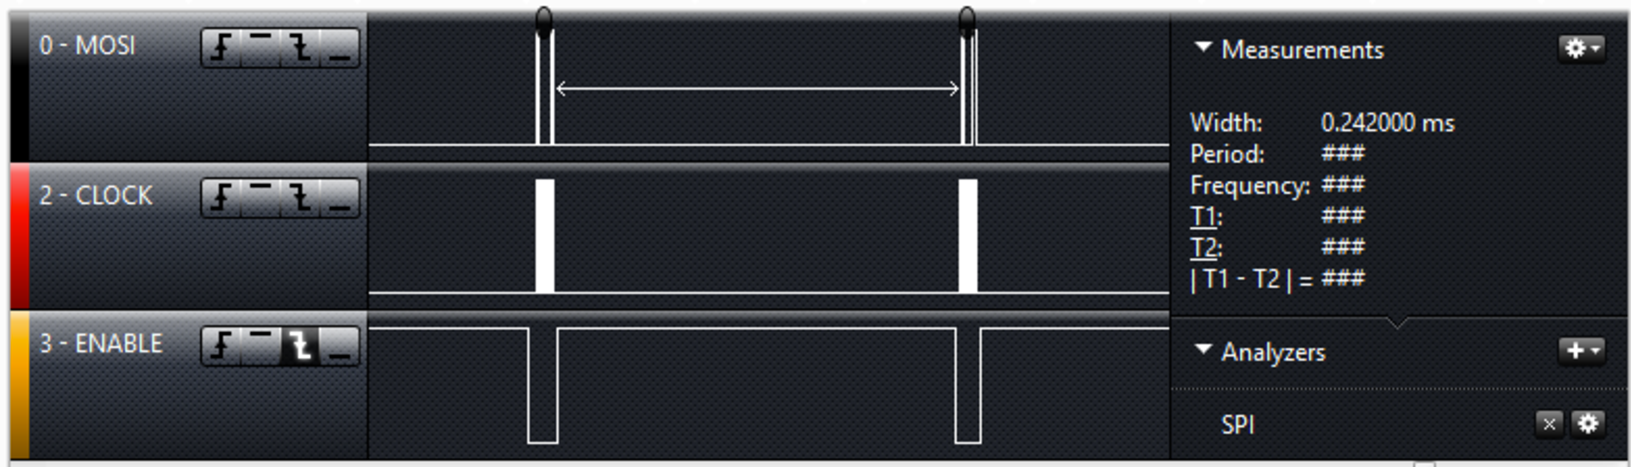
\includegraphics[width=0.90\textwidth]{filer/modultest/Billeder/mt_activate}}
\caption{Analysebillede for kommandoen aktiver}
\label{lab:mt_activate}
\end{figure}

Tabel \ref{table:mt_activate} viser hvad der ligger på \verb+MOSI+ transmissionen. Helt som forventet.

\begin{table}[H]
	\caption{Analysedata eksporteret til tabel}
	\centering
	\begin{tabular}{|l|c|c|}
		\hline 
		\textbf{Char nr} & \textbf{0} & \textbf{1} \\ 		
		\hline 
		\textbf{MOSI} & '\verb+A+' & '\verb+C+' \\ 
		\hline 
	\end{tabular} 
	\label{table:mt_activate}
\end{table}


% Deaktiver
\subsubsection*{Deaktiver}

Deaktiver testes med et testobjekt

\begin{lstlisting}[language=C]
int main(void){
	SPI_api test;
	test.deactivate(1); // 1 er et dummy enhedsnummer
}
\end{lstlisting}

\begin{figure}[H]
\centering
{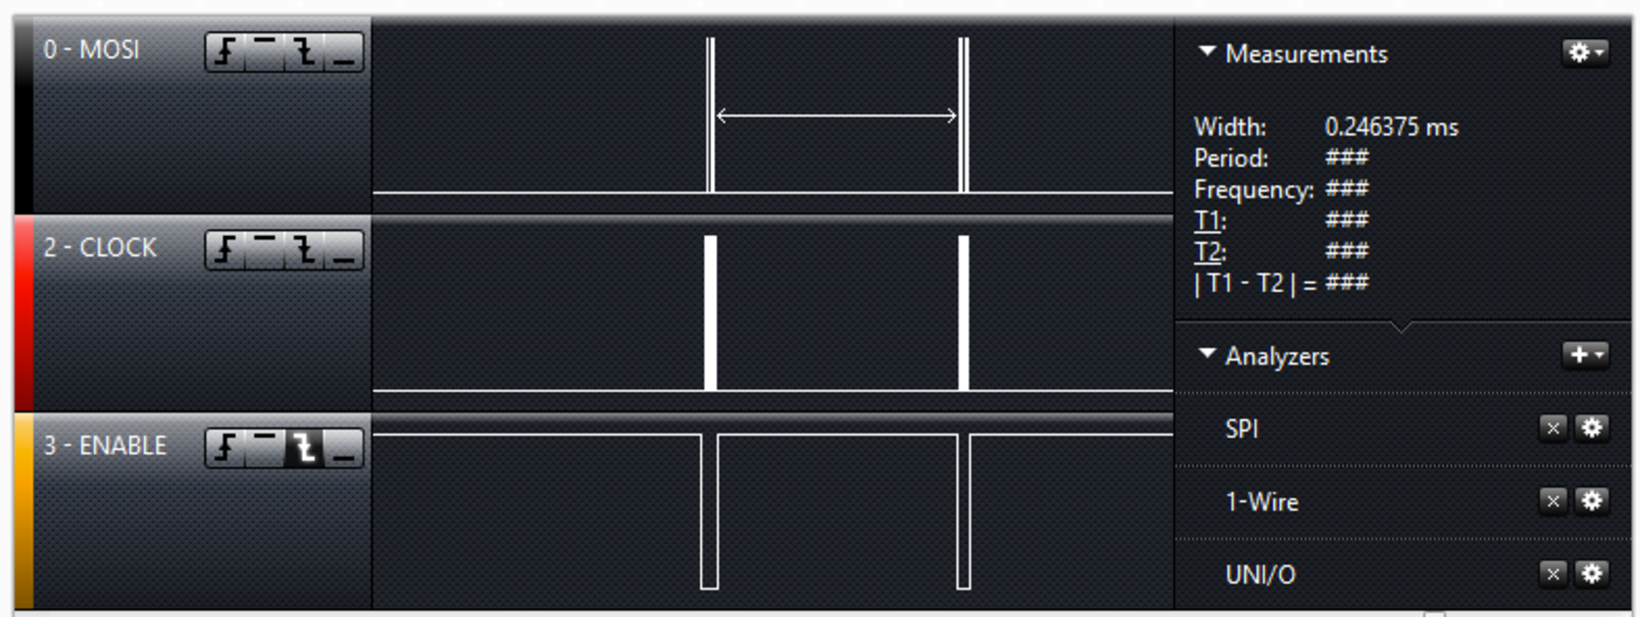
\includegraphics[width=0.90\textwidth]{filer/modultest/Billeder/mt_deactivate}}
\caption{Analysebillede for kommandoen deaktiver}
\label{lab:mt_deactivate}
\end{figure}

Tabel \ref{table:mt_deactivate} viser hvad der ligger på \verb+MOSI+ transmissionen. Helt som forventet.

\begin{table}[h]
	\caption{Analysedata eksporteret til tabel}
	\centering
	\begin{tabular}{|l|c|c|}
		\hline 
		\textbf{Char nr} & \textbf{0} & \textbf{1} \\ 		
		\hline 
		\textbf{MOSI} & '\verb+D+' & '\verb+C+' \\ 
		\hline 
	\end{tabular} 
	\label{table:mt_deactivate}
\end{table}


% Config
\subsubsection*{Config}
Config testes med 2 test-floats der sendes med config metoden.

\begin{lstlisting}[language=C]
int main(void){
	float tempTest = 100.1;
	float humiTest = 48;
	SPI_api test;
	
	test.config(1, tempTest, humiTest); // 1 er et dummy enhedsnummer
}
\end{lstlisting}

\begin{figure}[H]
\centering
{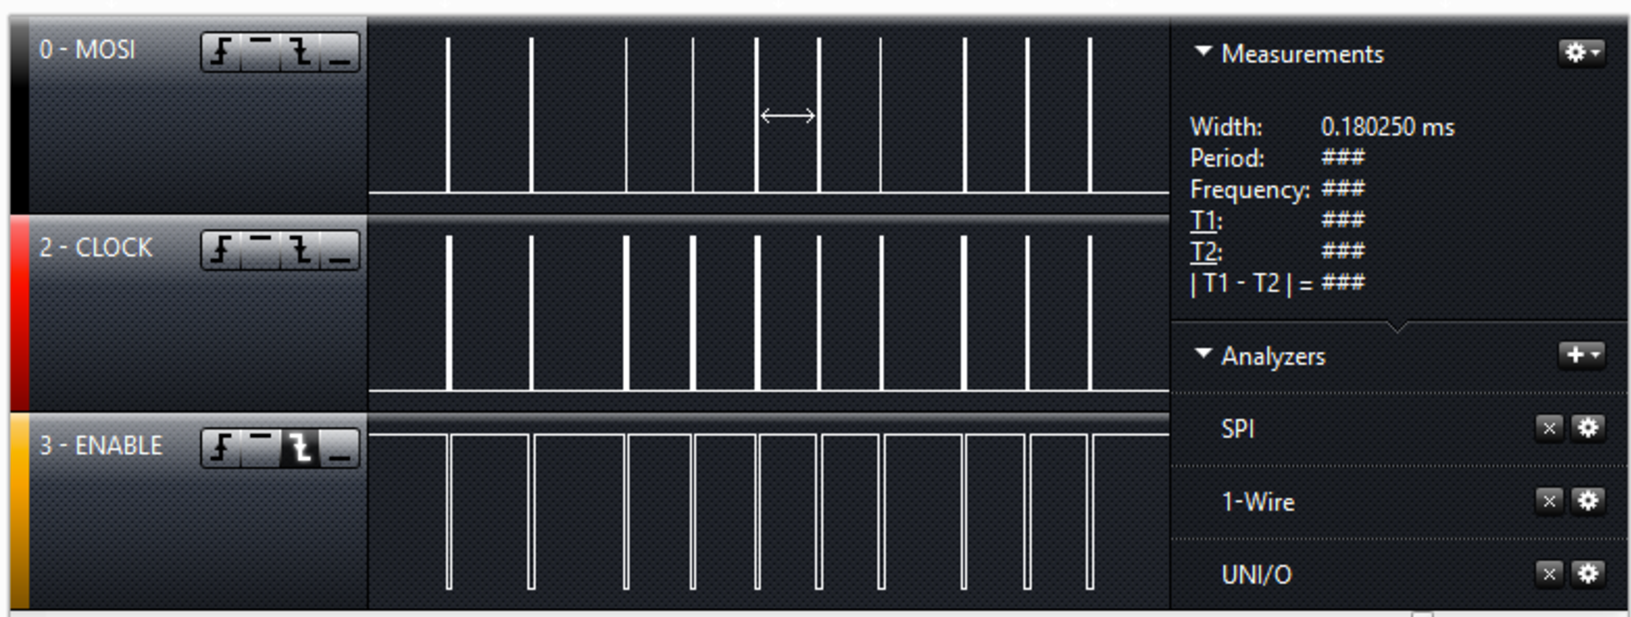
\includegraphics[width=0.90\textwidth]{filer/modultest/Billeder/mt_config}}
\caption{Analysebillede for kommandoen config}
\label{lab:mt_config}
\end{figure}

Tabel \ref{table:mt_config} viser hvad der ligger på \verb+MOSI+ transmissionen. Helt som forventet.

\begin{table}[H]
	\caption{Analysedata eksporteret til tabel}
	\centering
	\begin{tabular}{|l|c|c|c|c|c|c|c|c|c|c|}
		\hline 
		\textbf{Char nr} & \textbf{0} & \textbf{1} & \textbf{2} & \textbf{3} & \textbf{4} & \textbf{5} 
						 & \textbf{6} & \textbf{7} & \textbf{8} & \textbf{9}\\ 		
		\hline 
		\textbf{MOSI} & '\verb+P+' & '\verb+1+' & '\verb+0+' & '\verb+0+' & '\verb+.+' & '\verb+1+' 
						& '\verb+0+' & '\verb+4+' & '\verb+8+' & '\verb+C+' \\ 
		\hline 
	\end{tabular} 
	\label{table:mt_config}
\end{table}


% Verificer
\subsubsection*{Verificer}
Verify testes med et testobjekt og der sendes et 1-tal af sted til sammenligning med Enhedens enhedsnummer.

\begin{lstlisting}[language=C]
int main(void){
	SPI_api test;	
	test.verify(1);
}
\end{lstlisting}

\begin{figure}[H]
\centering
{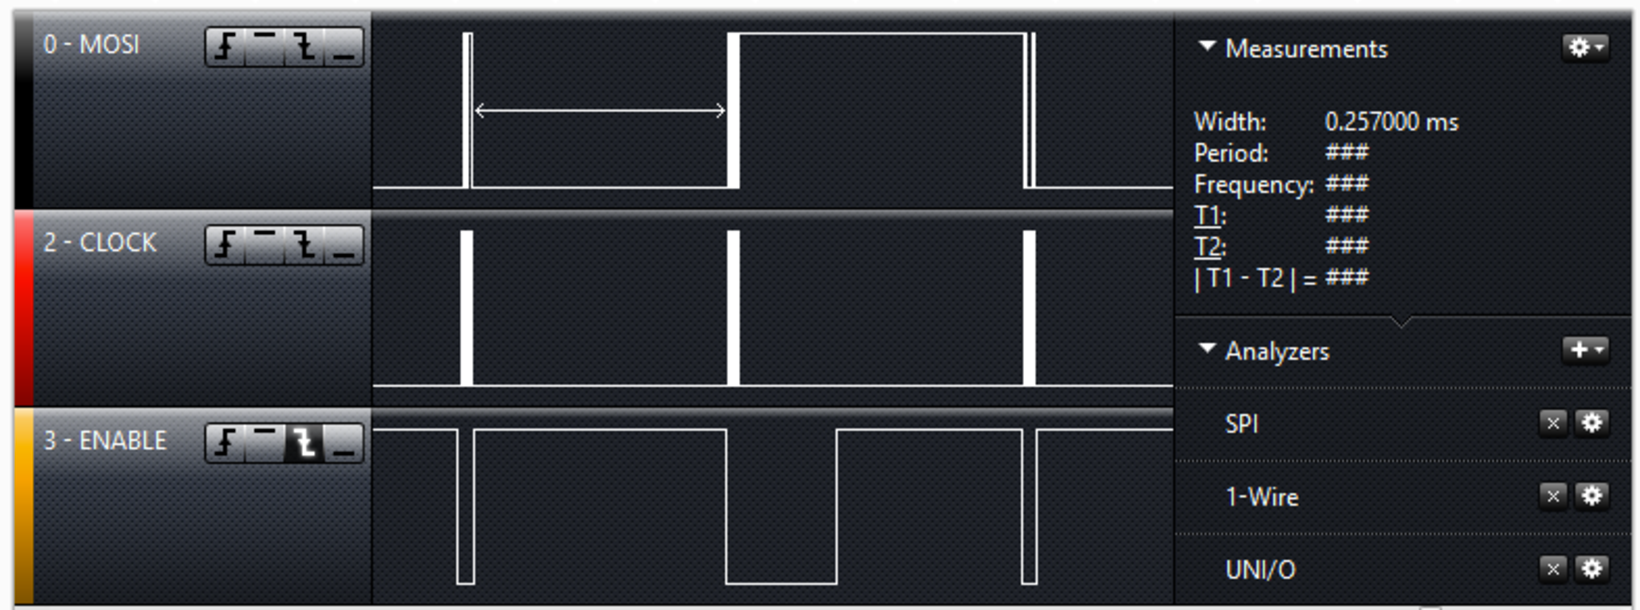
\includegraphics[width=0.90\textwidth]{filer/modultest/Billeder/mt_verify}}
\caption{Analysebillede for kommandoen verificer}
\label{lab:mt_verify}
\end{figure}

Da der i testen ikke er koblet en Enhed på, returneres der en fejl i debug-consollen i Eclipse, helt som forventet.

\verb+Not Verified: -12+

Tabel \ref{table:mt_verify} viser hvad der sendes på \verb+MOSI+ linjen, som forventet

\begin{table}[H]
	\caption{Analysedata eksporteret til tabel}
	\centering
	\begin{tabular}{|l|c|c|c|}
		\hline 
		\textbf{Char nr} & \textbf{0} & \textbf{1} & \textbf{2}\\ 		
		\hline 
		\textbf{MOSI} & '\verb+V+' & '\verb+R+'  & '\verb+C+'\\ 
		\hline 
	\end{tabular} 
	\label{table:mt_verify}
\end{table}

% Log

\subsubsection*{Log}
GetLog metoden testes med et test-objekt, men eftersom der læses på data fra Enheden har det ikke været muligt at teste metoden alene, den testes derfor først i integrationstesten af SPI, se afsnit \ref{section:spi_integrationstest}.

\subsection{Handler}

 Handleren testes i integrationstesten af SPI-kommunikationen, hvor Devkit8000 og PSoC kobles sammen med testprogrammer installeret.